\documentclass[11pt]{article}
\usepackage[final]{acl}
\usepackage{fontspec,xeCJK}
\setmainfont{Times New Roman}
\setCJKmainfont{SimSun}[AutoFakeBold=true]
\setCJKsansfont{SimHei}
\usepackage{microtype,amsmath,amssymb,booktabs,graphicx,array,multirow,xurl}
\graphicspath{{../figures/}}
\newcommand{\G}{\mathsf{G}}
\newcommand{\W}{\mathbf{W}}
\title{WELD：语言模型能多好地构建和调整动态工作流？}
\author{Zhixuan Liu \\ Northeastern University
\And Qi Yan\thanks{通讯作者。} \\ Northeastern University}
\begin{document}
\maketitle
\begin{abstract}
语言模型越来越多地决定智能体系统做哪些工作、如何合并结果，以及条件变化后需要修改什么。仅检查最终答案难以评价这些决策。本文提出可执行基准 WELD，将任务有效性、领域原生工作量、实际时间收益和选择性适应连接起来。基准包含五个场景、20 个来源簇、100 个父任务，每个任务具有初始、相关变化和无关变化三种条件。十个 API 模型产生 6,000 个阶段结果，另完成 8,874 次原生执行回放。在 5,006 对有效初始方案中，2,241 对存在工作量支配关系，372 对存在资源取舍；187 对方案的工具调用数相同，但主要工作量不同。中等任务中，在线时间节省落后于工作量节省，按父任务等权平均相差 31.6 个百分点；扣除本地准入等待后仍相差 14.5 个百分点，而原生回放往往兑现了节省。初始结果有效时，无关变化后的有效率为 99.3\%，相关变化后为 54.6\%。WELD 用成功工作、实际收益和维护行为共同刻画工作流有效性。
\end{abstract}

\section{引言}
工作流决定一个智能体系统读取什么、执行哪些测试、共享哪些结果，以及重复哪些工作。两个模型可以提交相同的正确答案，却采用不同的执行方案。一条查询既可以处理请求中的少量对象，也可以聚合整个数据库。复用一份观察既可以省去调用，也可以保留来自错误版本的结果。最终答案说明任务是否完成，工作流评价还需要说明这些工作是否被有效组织。

近期基准已经把工作流执行变成具体的评测对象。ClawArena-Team 固定工人池，通过任务、权限和模态路由的执行评分评价经理模型\citep{xiong2026clawarenateam}。这一设计使模型决策能够在工人受控时被研究。下一步问题位于实际执行内部：成功方案可能请求过多工作，局部节省可能不能按比例缩短完成时间，部分条件变化也可能破坏已有正确结果。经理层面的综合评分没有展开这三个关系。

本文研究\textbf{工作流有效性}：模型运行中决策、这些决策引发的工作，以及它们持续维持的有效结果之间的关系。测量需要保留工作量的领域含义。一次回归用例、一次数据库进度回调和一条遥测记录是不同资源。时间需要区分原生执行、模型交互和服务等待。适应需要从模型自己完成的状态开始，才能评价已有工作的复用与修复。

我们提出 WELD，即 Work, Execution, and Lifecycle Diagnostics。模型通过迭代接口创建并修改数据流，固定原生工人执行每个批次并返回中间观察。可执行任务契约同时检查提交结果与证据或应用状态。版本化产物、计划修订和实际事件把意图与行为连接起来，支持三个直接比较：正确方案需要多少工作；工作节省兑现了多少时间收益；已有正确方案如何响应相关与无关变化。

基准覆盖图检索、代码审查、数据库分析、遥测诊断和业务操作。100 个父任务来自 20 个来源簇，每个任务具有三个条件，每个模型独立生成两次。简单任务提供可比较的有效执行，中等任务保留批处理、范围选择、复用和多源整合决策。十模型实验共得到 6,000 个阶段结果和 8,874 次忠实原生回放。结果显示，正确率、工作量、在线收益和变化适应提供互补信息，WELD 将这些信息落实到同一套执行记录。

\section{相关工作}
\paragraph{工作流评价。}
WorFBench 构建多场景工作流任务，以子序列和子图匹配评价生成结果，并报告下游表现和时间\citep{qiao2025worfbench}。结构匹配不能说明另一种有效分解需要多少原生工作。FlowMind 将任务执行与工作流重建分离，并提出 FlowBench\citep{liu2026flowmind}。它提供了从执行到结构的生成方法；本文进一步比较已执行方案的资源及其后续修订。OrchBench 在给定 DAG 上评测任务分配和信息传递，通过确定性模拟返回质量、工期和 token 成本\citep{ren2026orchbench}。WELD 让模型选择实际调查，并测量原生操作和观察到的时间。

\paragraph{智能体评价。}
AgentBoard 提出细粒度进度率与多轮智能体分析工具\citep{agentboard}。子目标进展与完成这些目标所需的工作量是互补信息。AppWorld 提供可执行应用和允许多种解法的状态测试\citep{trivedi2024appworld}。WELD 采用结果验证，并在多个领域增加配对工作量测量和完成状态后的变化。ClawArena-Team 通过受控工人测量管理行为，包含权限、模态路由和任务结果\citep{xiong2026clawarenateam}；其费用分析已显示成本与质量可能分离。本文关注原生节省是否兑现为在线收益，以及变化后需要哪些新增工作。

\paragraph{效率与评价单位。}
\citet{agentsmatter} 主张联合评价准确率与成本，并改进留出集和复现纪律。BIRD 在真实数据库上评价 SQL 正确性和执行效率\citep{bird}。这些工作建立了效率评价的必要性。WELD 将领域工作向量、实际时间和更新行为连接到同一条工作流生命周期。本文的指标覆盖表按具体操作定义进行比较，并保留模拟量与实际执行量的区别。

\section{WELD：可执行测量}
\subsection{模型生成的动态数据流}
任务表示为 $(x,c,\mathcal O,V)$，分别为冻结的源世界、公开要求、允许算子和可执行验证器。每一轮，模型读取任务、当前节点、版本化观察和运行反馈，创建包含算子、参数和依赖的节点。参数可以引用先前产物。运行时执行一个批次后返回观察，模型再决定下一步调查、修改待执行范围、补充依赖或提交结果。

四个确定性工人槽运行领域算子，包括图遍历、源码读取、回归探针、只读 SQL、遥测聚合和本地应用状态变更。共享变换支持筛选、分组、投影、排序与聚合。模型既可以调用原生聚合算子，也可以组合底层操作。长输出即使在界面中被截断，完整内容仍可通过产物引用访问。

初始图、后续修订和真实执行事件分别保存。每份产物记录生产事件、输入产物、源版本和内容哈希。更新阶段继承完成检查点，历史工作保留身份，但不进入新增资源总量。图\ref{fig:designzh}展示执行和测量之间的联系。

\begin{figure*}[t]
\centering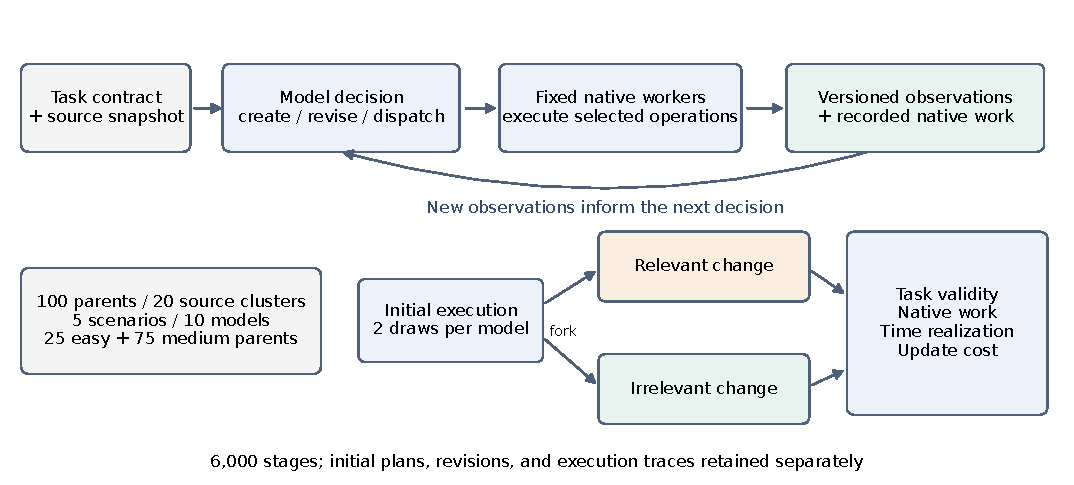
\includegraphics[width=.95\textwidth]{figure_0_experiment_design.pdf}
\caption{模型在批次之间读取观察并决定后续工作。相关变化和无关变化从相同检查点分叉；原生回放固定模型响应，改变工人容量。}
\label{fig:designzh}
\end{figure*}

\subsection{有效性和比较池}
对结果 $y$、观察 $E$ 和最终状态 $s$，定义
\begin{align}
Q_1&=\mathbf1[y,s\text{满足输出契约}],\\
Q_2&=\mathbf1[E,s\text{满足支持要求}],\\
\G&=Q_1Q_2.
\end{align}
只读任务验证必需值、对象或测试身份及观察的适用性；业务任务检查实际状态和保护条件。不同正确分解可以通过同一契约。冻结的等价性审计允许等价 SQL 和图访问方式。证据自动连接到执行产物，因而测量的是实际支持，而非引用格式。

所有计划阶段均进入无条件有效率分母，未提交计为零。工作与时间比较额外要求两个方案在相同父任务、初始条件和生成序号上均通过 $\G$。正确率与比较池同时报告，成功较少的模型既有较低质量分数，也提供较少有效比较。

\subsection{工作量、时间与收益}
设 $\mathcal E_\tau$ 为工作流中具有唯一身份的执行事件，则
\begin{equation}
\W(\tau)=\sum_{e\in\mathcal E_\tau}\mathbf w(e).
\end{equation}
向量坐标保留原生单位，包括图记录、回归用例、数据库进度回调、指标值、日志和链路行、业务记录和写入以及数据变换。失败和重试发生了工作就计入。模型请求使用独立台账，保存 token、费用回执、未知费用与重试。

如果全部原生坐标均不增加且至少一个严格减少，则方案 $a$ 在记录的工作量上支配 $b$：
\begin{equation}
\begin{aligned}
&\forall j\in J:W_j(a)\le W_j(b),\\
&\exists j\in J:W_j(a)<W_j(b).
\end{aligned}
\end{equation}
$J$ 包含该场景所有活跃原生坐标，排除模型请求。等量和资源取舍分别保留，不需要把用例、记录和写入换算为一个分数。

在线时间覆盖运行开始至完成，包含模型请求和本地准入等待。评分在之后执行。经理与工人区间并集分别为 $U_M,U_W$，重叠为 $O$，则
\begin{equation}
T=U_M+U_W-O+T_{\rm other}.
\end{equation}
我们另报告扣除本地准入等待的在线时间，服务端等待仍包含其中。原生回放复用保存的模型响应，不再次调用 API，在一和四个工人槽上各执行三次，以工人活动区间并集的中位数计时。

对工作量占优的低工作方案 $\ell$ 及高工作方案 $h$，预先指定场景主要坐标 $j_s$，定义
\begin{equation}
S_W=1-\frac{W_{j_s}(\ell)}{W_{j_s}(h)},\quad
S_T=1-\frac{T(\ell)}{T(h)}.
\end{equation}
两者差 $D=S_W-S_T$ 表示兑现差距。$0<S_T<S_W$ 即有收益但低于工作节省比例。配对要求主要工作量不同、分母为正、每阶段只有一次物理尝试；在线比较还要求采集批次和准入配置相同。

\subsection{选择性适应与新增代价}
从有效初始执行出发，对相关或无关变化 $u$，定义
\begin{equation}
A_u=\frac{\sum_{p,r}\G_{p,r,0}\G_{p,r,u}}
{\sum_{p,r}\G_{p,r,0}}.
\end{equation}
相关变化改变要求、版本或源状态；无关变化保持目标不变。两个分支继承同一检查点。仅新增事件计入 $\Delta\W,\Delta C,\Delta T$，完整路径只计算一次前缀。

独立前缀审计将旧答案和旧证据置于新条件下重新验证，区分答案需要改变、证据需要更新、二者均需改变以及均可复用。只读源版本变化时，验证器可以重新执行旧观察，判断其结果是否仍适用；这些验证工作独立记账，不归给模型。

\subsection{汇总与测量验收}
质量表分别报告五个场景的 $\G$，以及场景等权平均。每场景有 20 个父任务、三个条件、两次重复，因此总体宏平均等于每模型有效阶段数除以 600。工作、时间、适应和费用不混成加权总分。

配对观察共享父任务和模型结果。兑现差距先在父任务内部平均，再以父任务为单位进行 4,000 次 bootstrap，得到 95\% 百分位区间。适应分析还按场景内来源簇与簇内父任务重采样，并提供两两共同支持集和逐来源删除结果。

验收覆盖正例、错误身份、过期版本、等价表示和失败执行。最终审计核对逻辑阶段、物理请求和产物引用。8,874 次原生回放全部得到有效结果，且原生观察与工作向量与原记录一致。附录说明计数不变量与数学性质。

\section{任务集构建}
五个场景各包含 20 个父任务，其中简单五个、中等十五个。每个父任务生成初始、相关变化、无关变化三张卡片，共 300 张。每模型对每卡片生成两次。图\ref{fig:datazh}展示来源与改造过程。

\begin{figure*}[t]
\centering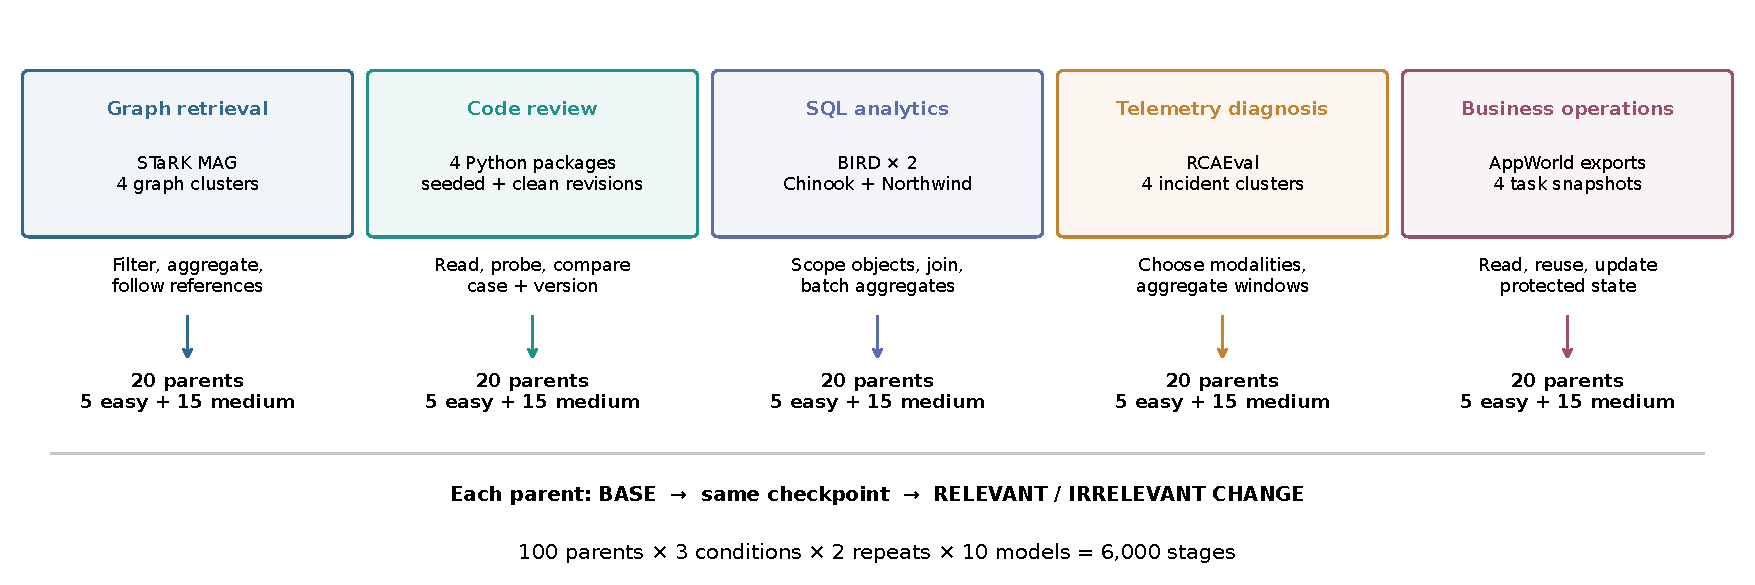
\includegraphics[width=\textwidth]{figure_4_dataset.pdf}
\caption{冻结来源、领域任务与条件分叉。每个场景具有四个来源簇和 20 个父任务。难度变化减少或增加输出负担，同时保留范围、批处理、复用和更新选择。}
\label{fig:datazh}
\end{figure*}

\paragraph{图检索。}
从 STaRK MAG 图构建组合查询\citep{stark}，使用已有共享切片以及 Stanford、MIT、东京大学三个机构邻域。保留作者发表记录闭包和论文引用。简单任务汇总一个作者的论文数、引用数和最高引用论文；中等任务组合作者并读取选定论文的参考文献。相关变化把年份范围从 2010--2014 扩展到 2000--2024。先过滤、广泛读取以及复用旧记录产生不同工作量。

\paragraph{代码审查。}
使用 Requests 2.32.5、ItsDangerous 2.2.0、packaging 25.0 和 python-dotenv 1.1.1\citep{requests,itsdangerous,packaging,dotenv}。围绕重定向与复制、时间边界、版本约束和解析行为，构建干净及人工植入变更的快照。公开测试契约提供预期行为，原生探针读取当前实现的行为。模型输出审查结论和精确失败用例身份。中等任务增加范围内用例和跨模块要求。相关变化替换实现版本。所有人工变更均保留来源标签。

\paragraph{数据库分析。}
BIRD 的 debit、financial 数据库以及 Chinook、Northwind 提供四个来源簇\citep{bird,birdminidev,chinook,northwind}。任务要求消费、区域贷款或客户采购等绑定对象的聚合结果。中等任务增加对象和字段。相关变化替换请求对象或修改一个值。模型可使用范围化聚合算子或只读 SQL，暴露批处理、广泛扫描和重复查询的工作差异。

\paragraph{遥测诊断。}
RCAEval 提供 Online Boutique 与 Train Ticket 的指标、日志和链路\citep{rcaeval}。原有 checkout 事件及三个新增服务事件组成四个来源簇。任务在公开分割时间前后比较指标均值比；中等任务增加链路时长比和日志匹配计数。相关变化移动分割点，原始遥测保持不变。真值来自这些可观察诊断量。

\paragraph{业务操作。}
四个 AppWorld 任务快照提供播放列表、用户和支付记录\citep{trivedi2024appworld}。我们将记录导出至本地确定性状态适配器，构建播放、离线下载和支付对账任务。更新改变时长、增加列表或计入部分支付。多个列表可以满足时长，既有下载可以复用，写入按成员替换请求金额。验证器检查实际效果及受保护状态。结果属于这套改造任务。

\paragraph{构建控制。}
冻结源数据分别生成公开任务卡与私有预期结果。要求明确对象身份、数值容差、状态义务及允许操作。参考执行检查可满足性，受控突变检查拒绝能力。20 个来源簇保留共享语料关系：MAG 邻域共享部分引用，AppWorld 快照共享生成数据。此前极复杂任务独立归档，不并入本轮主实验。

\section{实验设置}
十模型均使用相同任务接口和固定工人，每模型 600 个逻辑阶段。初始阶段最多 12 轮决策，更新最多八轮，每轮最多 8,192 输出 token，四个原生工人槽并行执行。采用端点默认采样，两次独立生成。开发阶段冻结各端点兼容的推理配置，正式请求使用 JSON 对象接口。格式失败、工具失败和未提交均保留在质量分母中。

各采集批次保留配置记录。历史模型与最终新增五模型使用相同任务契约和最终等价性规则。已确认传输中断按记录策略替换，错误答案不因结果不理想重跑。资源保留物理尝试，计时使用单次尝试及匹配采集条件。原生回放在共同离线批次完成；此前磁盘中断批次全部排除。最终得到 6,000 个主阶段和 8,874 次回放。

\section{结果}
\begin{table*}[t]
\centering\small\setlength{\tabcolsep}{5pt}
\begin{tabular}{lrrrrrrr}
\toprule
Model & Graph & Code & SQL & Telemetry & Business & All stages & Initial \\
\midrule
\multicolumn{8}{l}{\emph{Open-weight model families, served through APIs}}\\
DeepSeek V4 Pro 0813 & 29.2 & 34.2 & 70.0 & 61.7 & 29.2 & 44.8 & 58.5 \\
Kimi K2.6 & 52.5 & 48.3 & 78.3 & 67.5 & 65.0 & 62.3 & 76.5 \\
Qwen3.8 Flash & 84.2 & 40.0 & 88.3 & 65.8 & 56.7 & 67.0 & 79.5 \\
Gemma 4 31B & 86.7 & 23.3 & 98.3 & 66.7 & 63.3 & 67.7 & 80.5 \\
GLM-5.3 Flash & 97.5 & 63.3 & 92.5 & 86.7 & 98.3 & 87.7 & 92.0 \\
MiniMax M3 & 0.0 & 10.0 & 5.8 & 20.8 & 6.7 & 8.7 & 9.5 \\
\midrule
\multicolumn{8}{l}{\emph{Closed-model APIs}}\\
Gemini 3.8 Flash & 100.0 & 71.7 & 99.2 & 70.8 & 100.0 & 88.3 & 98.0 \\
Gemini 3.7 Flash & 100.0 & 68.3 & 100.0 & 76.7 & 100.0 & 89.0 & \textbf{98.5} \\
Grok 4.3 & 41.7 & 18.3 & 57.5 & 49.2 & 17.5 & 36.8 & 48.5 \\
GPT-6 Luna & 98.3 & 72.5 & 100.0 & 98.3 & 96.7 & \textbf{93.2} & 98.0 \\
\bottomrule
\end{tabular}
\caption{联合有效率（\%）。各场景每模型 120 阶段，总计 600 阶段；初始列为 200 阶段。总体为场景等权平均。粗体标记总体与初始最高值。所有模型均通过 API 调用。}
\label{tab:zh_quality}
\end{table*}
\subsection{有效性提供直接比较的基础}
全部阶段有 3,873/6,000 通过 $\G$；初始为 1,479/2,000，即 74.0\%，100 个父任务全部具备有效配对。图检索、代码、数据库、遥测和业务的初始有效数分别为 291、235、343、347、263，分母均为 400。

初始有效性与生命周期有效性揭示不同表现。Gemini 3.7 Flash 的初始有效数最高，为 197/200；GPT-6 Luna 的总体有效数最高，为 559/600，相关更新恢复 165/196。GLM-5.3 Flash 初始通过 184 个，相关更新恢复 150 个。MiniMax M3 提交了全部 600 阶段，但初始只有 19 个有效结果。交付率说明接口完成，不能替代任务完成。

\subsection{发现一：相同有效结果隐藏不同工作量}
\begin{figure*}[t]
\centering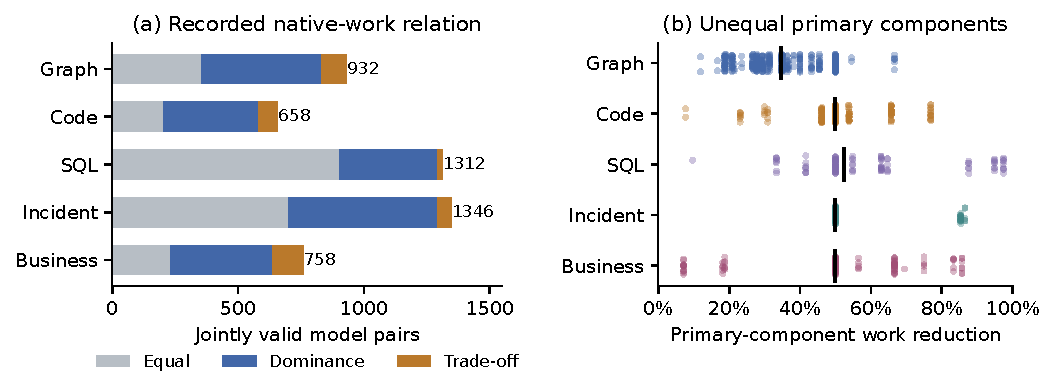
\includegraphics[width=\textwidth]{figure_1_correct_work_differences.pdf}
\caption{5,006 对有效初始执行的原生工作量。左侧显示完整向量上的等量、支配和取舍；右侧显示场景主要坐标差异。单坐标节省需与完整向量关系共同解释。}
\end{figure*}
1,479 个有效初始执行产生 5,006 对跨模型比较。其中 2,393 对向量相等，2,241 对存在支配，372 对存在资源取舍。正确性确定了比较对象，但没有决定其工作量。

3,619 对方案的工具调用数相同，其中 187 对的主要原生工作量不同，涉及 29 个父任务。在客户审计 A14 中，Qwen3.8 Flash 和若干正确替代方案都只调用一次原生工具，但分别触发 39 和两次 SQLite 进度回调。这个测量代理相差 19.5 倍。“一次查询”会抹去数据库实际处理量的区别。

372 对资源取舍同样有价值：减少一种工作可能增加另一种工作。WELD 先报告向量关系，再计算主要坐标节省，因此可以根据明确资源偏好判断哪个有效方案更好。

\subsection{发现二：原生节省与在线收益分离}
\begin{figure*}[t]
\centering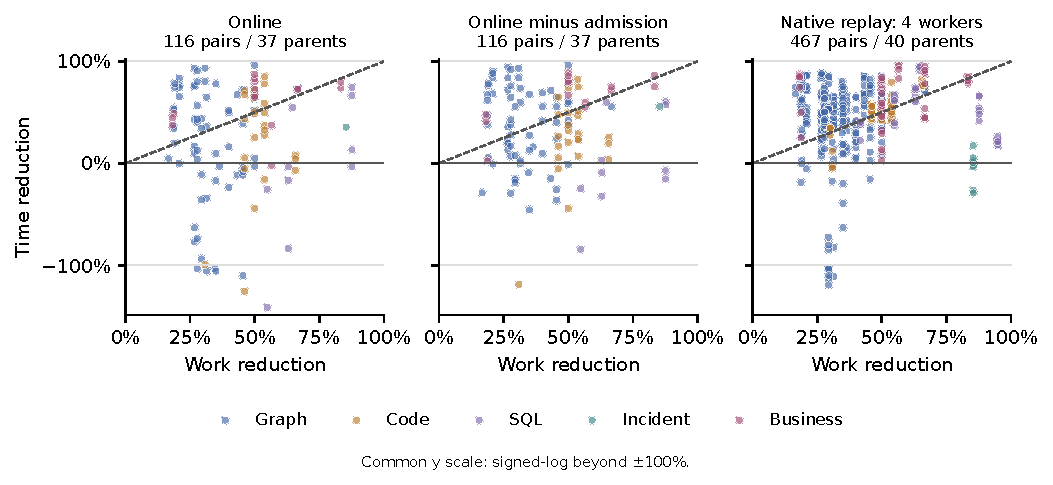
\includegraphics[width=\textwidth]{figure_2_work_to_time.pdf}
\caption{中等任务的工作量节省与时间节省。在线比较为 37 个父任务上的 116 对；四工人原生回放为 40 个父任务上的 467 对。对角线表示等比例兑现；线上方与下方分别表示更多和更少的时间收益。原生时间采用工人活动区间并集。}
\end{figure*}
116 对工作量占优方案满足在线采集控制。其中 29 对有正向但不足比例的时间节省，33 对时间节省为零或负，54 对至少等比例兑现。父任务等权平均兑现差距为 31.6 个百分点，95\% 区间为 13.7--52.4。扣除本地准入等待后，差距缩至 14.5 个百分点，区间为 3.7--26.3。

原生层呈现不同结果。467 对四工人回放中，108 对正向衰减，27 对无正收益，332 对至少等比例兑现。父任务等权平均差距为 $-6.0$ 个百分点，区间为 $[-13.7,2.9]$，不表现为总体正向衰减。

进一步在相同 116 对方案上比较两个计时域，原生时间节省比扣除准入后的在线节省高 24.2 个百分点，区间为 13.9--34.5。测量把差异定位在本地执行与交互完成之间。模型请求、服务等待和运行时协调能够消耗原生收益，因此评价需要同时关注批处理、交互频率与请求工作量。

\subsection{发现三：保持比修复容易}
\begin{figure*}[t]
\centering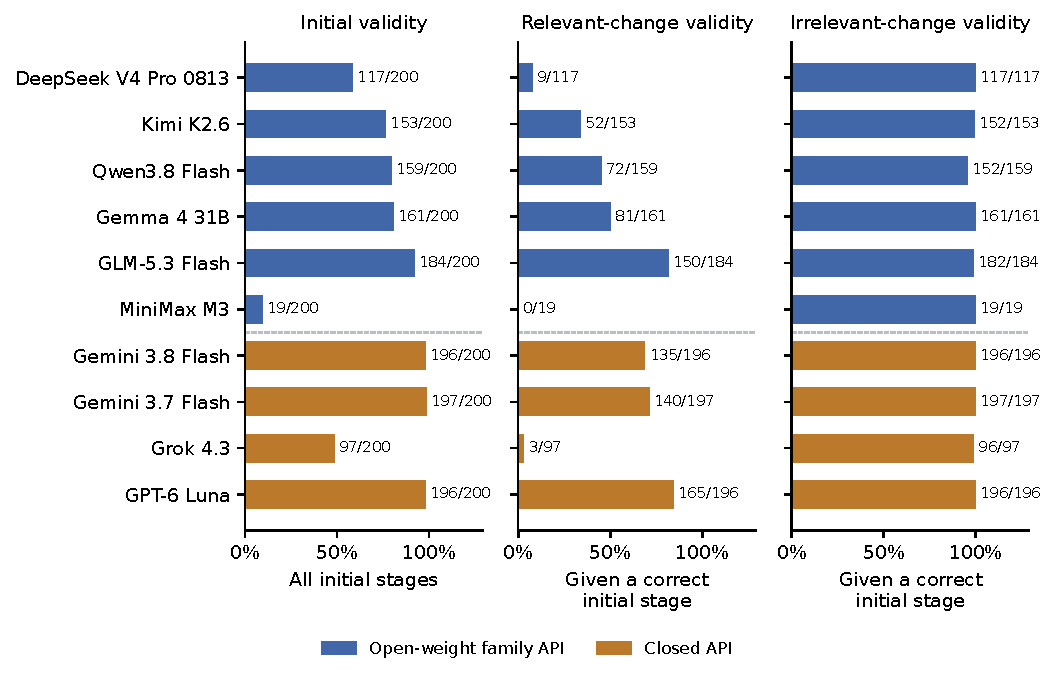
\includegraphics[width=\textwidth]{figure_3_selective_adaptation.pdf}
\caption{初始有效性及从有效初始状态出发的适应。相关和无关变化使用图中标出的初始有效分母。开源模型家族 API 与闭源 API 分组展示。各模型条件比例使用各自比较池，两两共同支持集另行提供。}
\end{figure*}
1,479 个有效初始状态中，无关变化保留 1,468 个有效结果，即 99.3\%；相关变化仅得到 807 个，即 54.6\%。是否需要真正修订，显著改变了后续表现。

前缀审计进一步拆解修订需求。1,183 次变化同时使旧答案和证据不足，其中 585 次恢复。228 次保留充分证据但需要改变答案，其中 168 次恢复。28 次答案仍然正确却需要新证据，只有 14 次恢复。40 次前缀仍完全有效的情况均保持有效。答案稳定与证据稳定是不同属性。

相关更新中有 632 次没有新原生调用，仅 34 次有效；无关更新中则有 1,429 次不新增原生调用且保持有效。相同的“没有继续调用工具”，既可能是合理复用，也可能是修复失败，其含义由变化后的契约和证据决定。

Gemini 3.7 和 3.8 Flash 初始有效率接近，分别为 98.5\% 和 98.0\%，相关更新有效率为 71.1\% 和 68.9\%。Luna 初始为 98.0\%，相关更新为 84.2\%；GLM 初始为 92.0\%，相关更新为 81.5\%。各条件比较池不同，配套数据提供共同支持集、来源重采样和逐来源删除分析。

\section{讨论与结论}
WELD 将工作流有效性落实为三个可观察关系：有效结果对应不同工作向量；原生节省可以在执行层兑现，却在线上被削弱；已完成工作流可以应对通知，却在真正变化后修复失败。每个关系都把模型决策与执行后果相连。

这些测量给出具体改进目标。模型可以学习按请求对象收缩操作范围、合并兼容调查、减少执行价值有限的交互。版本感知策略可以区分重算答案、取得新证据和保留适用状态。训练与系统优化因而能够针对观测到的失败类型，同时检查有效性和新增代价。

本文贡献是相互连接的测量协议及可执行基准：任务级验证、原生工作画像、配对计时和完成状态后的适应。十模型实验说明，评价构建和维护动态工作流的模型，需要同时保留这四类信息。

\section*{局限}
WELD 使用人工构建任务和确定性工人，结果对应当前接口与端点配置。注册代码探针、聚合辅助算子和本地业务状态适配器使要求可执行，也限定了行动空间。20 个来源簇共享部分语料，两次生成提供的模型内采样有限。在线计时控制已记录的采集配置，仍保留服务端和网络波动。固定响应回放测量已生成决策的原生执行。支配关系依赖已记录坐标，SQLite 进度回调是粗粒度代理。全部十模型共同通过初始验证的交集仅八个父任务--重复单元，因此条件比较需要同时报告支持集。

\section*{伦理与复现}
研究使用公开代码、基准记录和生成的应用数据。人工植入变更明确标记，支付和播放操作在隔离本地状态中执行。冻结来源记录保留许可证与归属。复现包包括任务卡、验证器、模型配置、物理尝试索引、结果表、回放检查和可编辑矢量图；不含凭据及本地账户配置。

\bibliography{references}
\bibliographystyle{acl_natbib}
\clearpage\appendix
\section{计数性质与指标定义}
\paragraph{事件身份。}
每次物理请求和执行事件具有唯一身份。新增事件集合为 $N$ 时，增量工作为 $\Delta\W=\sum_{e\in N}\mathbf w(e)$。重复读取同一日志只计算一次；实际重试产生新的事件身份，再次计入。导入前缀保留历史消耗并将新增消耗置零，因此完整路径满足 $\W_{0\rightarrow u}=\W_0+\Delta\W_u$。

\paragraph{单位不变性。}
对坐标 $j$ 使用正数 $a_j$ 改变单位，同时乘两个方案的对应坐标，不改变支配不等式，也不改变 $1-a_jW_j(\ell)/(a_jW_j(h))$。这解释了为何可以保留异质原生单位，不必加权成总分。不同资源的代价偏好仍由使用场景决定。

\paragraph{时间可加关系。}
模型与工人活动并集满足容斥关系 $|I_M\cup I_W|=U_M+U_W-O$。从经过时间减去活动并集得到其他开销。并行工人时长之和不作为墙钟时间。原生回放采用 $|I_W|$，在线采用运行开始至完成的经过时间；验证和证据重执行另记账。

\paragraph{数据库工作代理。}
SQLite 每 1,000 条虚拟机指令触发一次进度处理器。历史字段名为 \nolinkurl{sqlite_vm_steps_lower_bound}，本文以回调数或其乘 1,000 的值作为工作代理。短查询可以为零，准备阶段及数据库版本也会影响回调行为，因此不将其写成精确指令数。A14 的 19.5 倍是 39/2 次回调之比。

\paragraph{指标分工。}
五场景主要工作量坐标依次为图论文记录读取数、原生回归用例数、SQLite 进度工作代理、指标值读取数和业务记录读取数。其余原生坐标仍全部进入支配判断。主要坐标分母为零时不计算节省比例，底表保留绝对值。
交付率为已提交并评分阶段数除以计划阶段数。$Q_1$ 检查输出契约，$Q_2$ 检查证据和状态，$\G$ 为二者合取。工作量为事件求和向量，支配关系保留资源取舍。$S_W,S_T,D$ 比较指定计时域中的工作和收益。$A_{\rm rel},A_{\rm irr}$ 测量有效前缀后的修复和保持。增量工作、模型请求、时间与费用说明更新代价。前缀审计区分答案变化、证据刷新和可复用状态。

\section{来源和改造细节}
\paragraph{图数据。}
STaRK 冻结版本为 \nolinkurl{88269e23e90587f99476c5dd74e235a0877e69be}。原切片有 16,550 个节点和 149,765 条边；Stanford、MIT、Tokyo 切片分别有 16,058/142,401、14,376/126,927、13,167/120,386 个节点/边。扩展过程在指定机构中按种子抽取作者，保留发表记录和外向引用。焦点作者与原集合不重叠，引用节点有重叠。四簇分配 8/4/4/4 个父任务。

\paragraph{代码数据。}
Requests 固定在 \nolinkurl{b25c87d7cb8d6a18a37fa12442b5f883f9e41741}，ItsDangerous 固定在 \nolinkurl{096c8d42545d3b68ea21a4f890fb2b2d8979c0bd}。packaging 和 python-dotenv 使用发布的 25.0 与 1.1.1 源码包，并记录 SHA-256。四簇分别分配 4/4/6/6 个父任务。原始、植入和修复快照独立保存，公开预期与当前观察分离。用例绑定包、检查名、用例名和版本；有效结论要求精确指出范围内失败项。

\paragraph{关系数据。}
BIRD debit 与 financial 各四个父任务，Chinook 与 Northwind 各六个。消费任务聚合指定年份和客户；贷款任务聚合地区与状态；采购任务统计去重订单数、行数量和行金额，Northwind 应用折扣。相关变化改变对象集或受控数据值。原生汇总函数与等价只读 SQL 都可以通过验证。

\paragraph{遥测数据。}
RCAEval 扩展文件固定版本为 \nolinkurl{afeacb11bcc94dadfd1c8f483ee4377b2b8b614e}。原 checkout 簇八个父任务，currency CPU、product-catalog delay 和 Train Ticket order CPU 各四个。保留指标、日志、链路和注入时间。公开切分点及过滤条件确定期望量，相关卡片只移动切分点。任务评价源遥测派生的诊断报告。

\paragraph{应用数据。}
四份 AppWorld 导出来自 \nolinkurl{b0a8eae_1}、\nolinkurl{22cc237_1}、\nolinkurl{3fcc458_1}、\nolinkurl{90adc3f_1}，父任务分配为 4/4/6/6。后两份分别包含六/四个播放列表、32/43 个支付请求和各 106 条用户记录。适配器在导出记录上实现本地状态变化：播放允许任一满足时长的列表，下载保持既有集合，支付按成员身份替换为 $\max(0,\mathrm{share}-\mathrm{paid})$。验证器检查最终状态。

\section{模型配置与验收}
全部模型通过 OpenRouter 调用，记录 provider、量化信息及请求参数。六个端点按开源模型家族归组，四个归为闭源 API；Qwen3.8 Flash 是日志中的生产端点，未绑定到某个公开检查点。最终新增 Grok 4.3、MiniMax M3、Gemini 3.7 Flash、GPT-6 Luna、GLM-5.3 Flash。Mistral Small 4 在正式阶段开始前持续限流，由 GLM 替换。

开发阶段冻结 JSON 对象和推理设置：GLM、Gemini 3.7、Luna 使用低推理，Grok 和 MiniMax 关闭推理。早期模型使用记录的兼容配置。全体保持相同原生工人和任务预算。在线配对匹配采集组及准入段，GLM 延后采集单列一组。原生回放在共同批次执行，Python 为 3.13.4，SQLite 为 3.49.1。

任务层验收通过 784 项，扩展契约验收通过 19 项，等价证据验收通过 11 项。非对象答案保护使 20 个畸形例子均被拒绝，并保留正常评分分支。等价性审计恢复两个 MiniMax 有效阶段，不改变模型响应及轨迹。四条传输错误占位记录不算模型 JSON 格式错误，仍保留于物理台账。

新增五模型有 3,000 个逻辑阶段、3,008 个物理阶段尝试；2,994 个逻辑阶段提交并评分，六个没有提交。四个物理请求保留未知费用预约。质量、交付和传输状态独立保存；最终 6,000 个逻辑阶段全部具有终态记录。

\section{补充结果与分母}
\begin{table*}[t]
\centering\small\setlength{\tabcolsep}{5pt}
\begin{tabular}{lrrrrrr}
\toprule
Model & Submitted & $Q_1$ & $\G$ & Initial $\G$ & Related $\G$ & Irrelevant $\G$ \\
\midrule
DeepSeek V4 Pro 0813 & 600/600 & 295/600 & 269/600 & 117/200 & 9/117 & 117/117 \\
Kimi K2.6 & 596/600 & 397/600 & 374/600 & 153/200 & 52/153 & 152/153 \\
Qwen3.8 Flash & 575/600 & 410/600 & 402/600 & 159/200 & 72/159 & 152/159 \\
Gemma 4 31B & 571/600 & 458/600 & 406/600 & 161/200 & 81/161 & 161/161 \\
GLM-5.3 Flash & 600/600 & 550/600 & 526/600 & 184/200 & 150/184 & 182/184 \\
MiniMax M3 & 600/600 & 97/600 & 52/600 & 19/200 & 0/19 & 19/19 \\
Gemini 3.8 Flash & 599/600 & 531/600 & 530/600 & 196/200 & 135/196 & 196/196 \\
Gemini 3.7 Flash & 600/600 & 537/600 & 534/600 & 197/200 & 140/197 & 197/197 \\
Grok 4.3 & 594/600 & 270/600 & 221/600 & 97/200 & 3/97 & 96/97 \\
GPT-6 Luna & 600/600 & 563/600 & 559/600 & 196/200 & 165/196 & 196/196 \\
\bottomrule\end{tabular}
\caption{精确分母。Submitted 表示已提交并评分；最后两列以初始有效为条件，因此不是相应 200 个更新阶段的无条件有效数。}
\label{tab:zh_counts}\end{table*}
\begin{figure*}[t]
\centering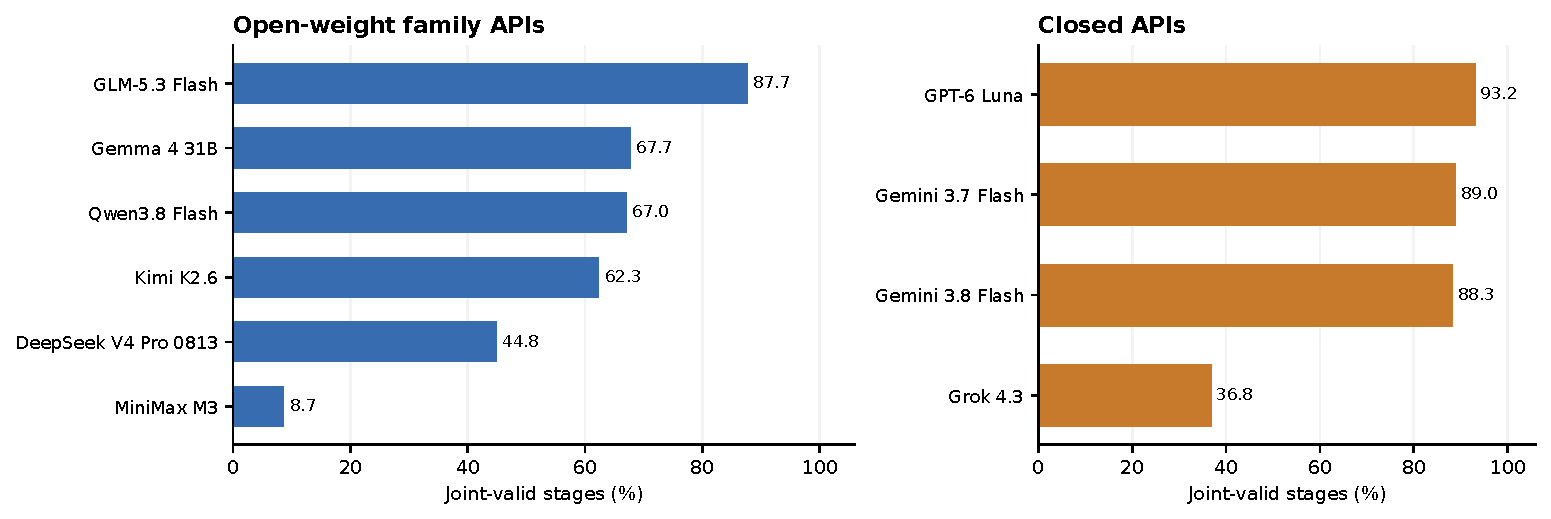
\includegraphics[width=.96\textwidth]{figure_5_validity.pdf}
\caption{按端点家族分组的描述性质量排行。分数为 600 个阶段的有效率；不合并工作量、时间及适应指标。}
\end{figure*}

初始、相关和无关条件的无条件有效数分别为 1,479、862、1,532，分母均为 2,000。条件更新比较中，相关与无关有效数分别为 807、1,468，分母为 1,479。差异来自无条件更新还包含初始无效状态的继续执行。

中等任务一工人回放中，121/467 对正向衰减，14/467 对无正收益，332/467 对至少等比例兑现，父任务等权差距为 $-7.9$ 个百分点，区间 $[-15.6,1.0]$。四工人相应为 108、27、332 对，平均差距 $-6.0$ 个百分点。

相同 116 对方案中，四工人原生节省比在线节省高 41.3 个百分点，区间 24.4--61.1；去掉本地准入后为 24.2 个百分点，区间 13.9--34.5。统计先在父任务内部平均，再在 37 个父任务间平均。

来源感知适应分析先在父任务内平均有效重复，再做场景内来源簇和父任务重采样。Luna 的相关更新父任务等权估计为 83.3\%，区间 76.7--89.7；GLM 为 81.1\%，区间 74.0--87.7。这与按有效重复数直接合并略有不同。全部十模型共同通过的初始交集仅八个父任务--重复单元，因此另提供每对模型的共同支持集。

\section{相关工作覆盖映射}
\begin{table*}[t]
\centering\small
\setlength{\tabcolsep}{3pt}
\begin{tabular}{lccccc}
\toprule
Evaluation & Executed outcome & Native work vector & Work--time pairing & Relevant updates & Valid-prefix cost\\
\midrule
WorFBench & $\circ$ & -- & -- & -- & --\\
FlowBench / FlowMind & $\checkmark$ & -- & -- & -- & --\\
AgentBoard & $\checkmark$ & -- & -- & -- & --\\
AppWorld & $\checkmark$ & -- & -- & -- & --\\
ClawArena-Team & $\checkmark$ & -- & -- & $\checkmark$ & --\\
OrchBench & $\circ$ & $\circ$ & $\circ$ & -- & --\\
\textbf{WELD} & $\checkmark$ & $\checkmark$ & $\checkmark$ & $\checkmark$ & $\checkmark$\\
\bottomrule
\end{tabular}
\caption{按本文操作定义映射的已报告测量。勾选为直接覆盖，圆圈为相关但测量域不同，横线为未单独报告该协议。Native work vector 保留领域单位；Work--time pairing 配对比较有效方案的原生工作与实际时间；Valid-prefix cost 测量有效完成前缀后的新增代价。}
\label{tab:zh_coverage}
\end{table*}

WorFBench v3 以结构匹配为主，并报告下游执行及计时；FlowMind v1 评价执行与重建工作流，包含 token 和工具分析；AgentBoard 报告进度和过程分析；AppWorld 通过应用状态检验结果。ClawArena-Team v2 具有执行评分、分阶段变化、权限及模态指标和使用量分析。OrchBench v1 通过确定性模拟测量质量、工期和 token。矩阵按照本文操作定义映射，对模拟域或粒度不同的量标记部分覆盖。最后一列要求从已验证完成前缀测量新增成本，并有相关/无关对照。

\section{复现材料}
底表包含 6,000 个阶段、5,006 对初始比较、各工作坐标、计时资格、前缀审计、适应比较池与来源敏感性分析。绘图代码直接使用这些表。完整研究归档索引初始计划、修订、观察、物理尝试及不可变源快照。任务卡和验证器代码独立保留。正文采用最终审计数值，开发探针和早期极复杂先导实验单独归档。

\end{document}
